\documentclass{beamer}

\newtheorem{conjecture}{Conjecture}
 \newcommand{\bconj}[1]{\begin{conj}#1\end{conj}}
\newtheorem{mconj}{Metaconjecture}

\newtheorem{prop}{Proposition}
 \newcommand{\bprop}[1]{\begin{prop}#1\end{prop}}
\newtheorem{lem}{Lemma}
 \newcommand{\blem}[1]{\begin{lem}#1\end{lem}}


\newtheorem{guess}{Guess}
 \newcommand{\bguess}[1]{\begin{guess}#1\end{guess}}
%\newtheorem{corollary}{Corollary}



\usepackage{tikz,framed, amsrefs, amsthm,  wrapfig,color}
\tikzstyle{every node}=[circle, draw, fill=black!50,
                        inner sep=0pt, minimum width=4pt]
\tikzstyle{dot}=[circle, draw, fill=black,
                        inner sep=0pt, minimum width=2pt]
\tikzstyle{lblvertex}=[fill=white, inner sep = 1pt, font=\small]
\tikzstyle{lblvertex2}=[fill=white, inner sep = 1pt, font=\tiny,circle, draw]
\tikzstyle{lblvertex3}=[fill=white, inner sep = 1pt, font=\tiny,circle, draw = black!25]
\tikzstyle{words} =[rectangle, draw=none, fill=none, black]
\newcommand{\bframe}[2]{\begin{frame}{#1}#2\end{frame}}
\newcommand{\bfig}[2]{\begin{figure}#1\caption{#2}\end{figure}}


\usetheme{CambridgeUS}
\setbeamertemplate{navigation symbols}{}
\usecolortheme[RGB={216,30,5}]{structure}
\AtBeginSection[] % "Beamer, do the following at the start of every section"
{
\begin{frame}<beamer>
\frametitle{Outline} % make a frame titled "Outline"
\tableofcontents[currentsection] % show TOC and highlight current section
\end{frame}
}

\title{Connected matchings in graphs}
\author{Chris Caragianis}
\institute[U of L]{ Department of Mathematics\\ University of Louisville\\ Louisville, KY 40292\\[1ex]
   \texttt{cjcara01@louisville.edu} }



\begin{document}

\bframe{Picture of a non-inert, bisimplicial edge}{
\pause
\begin{center}
\begin{overprint}
	\onslide<2>\hspace{4.5cm}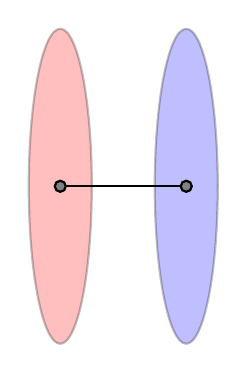
\begin{tikzpicture}[thick,scale=0.4]

\draw[fill = red, opacity = 0.25]  (-2,0) ellipse(1 and 5);

\draw[fill = blue, opacity = 0.25] (2,0) ellipse (1 and 5);

\draw (-2,0) node[]{}
	edge[] (2,0);
\draw (2,0) node[]{};

\end{tikzpicture}
	\onslide<3>\hspace{4.5cm}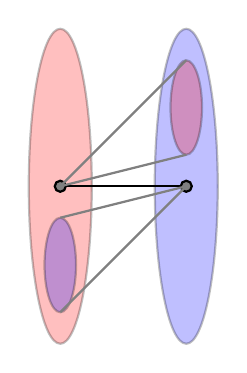
\begin{tikzpicture}[thick,scale=0.4]

\draw[fill = red, opacity = 0.25]  (-2,0) ellipse(1 and 5);
\draw [fill = blue, opacity = 0.25](-2,-2.5) ellipse (0.5 and 1.5);
\draw[fill = blue, opacity = 0.25] (2,0) ellipse (1 and 5);
\draw[fill = red, opacity = 0.25] (2,2.5) ellipse (0.5 and 1.5);
\draw (-2,0) node[]{}
	edge[] (2,0);
\draw (2,0) node[]{};

\draw[color = gray] (-2,0)--(2,4);
\draw[color = gray] (-2,0)--(2,1);
\draw[color = gray] (2,0)--(-2,-1);
\draw[color = gray] (2,0)--(-2,-4);
\end{tikzpicture}
	\onslide<4>\hspace{4.5cm}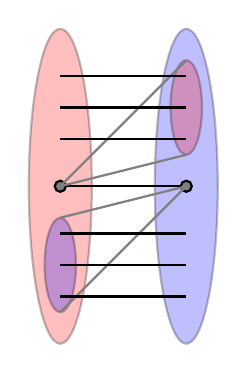
\begin{tikzpicture}[thick,scale=0.4]

\draw[fill = red, opacity = 0.25]  (-2,0) ellipse(1 and 5);
\draw [fill = blue, opacity = 0.25](-2,-2.5) ellipse (0.5 and 1.5);
\draw[fill = blue, opacity = 0.25] (2,0) ellipse (1 and 5);
\draw[fill = red, opacity = 0.25] (2,2.5) ellipse (0.5 and 1.5);
\draw (-2,0) node[]{}
	edge[] (2,0);
\draw (2,0) node[]{};

\draw[color = gray] (-2,0)--(2,4);
\draw[color = gray] (-2,0)--(2,1);
\draw[color = gray] (2,0)--(-2,-1);
\draw[color = gray] (2,0)--(-2,-4);

\draw (-2,3.5)--(2,3.5);
\draw (-2,2.5)--(2,2.5);
\draw (-2,1.5)--(2,1.5);
\draw (-2,-3.5)--(2,-3.5);
\draw (-2,-2.5)--(2,-2.5);
\draw (-2,-1.5)--(2,-1.5);
\end{tikzpicture}
\end{overprint}
\end{center}

}



\end{document}